%!TEX root = ../luanvan.tex
\chapter{Kết quả thực nghiệm}
\section{Mạng blockchain}

Mạng Blockchain được cài đặt  trên máy tính cá nhân có cấu hình như sau:
\begin{itemize}
\item CPU: Intel(R) Core(TM) i3-10100F 3.00 GHz
\item RAM: 8 GB
\item Hard Disk: 120 GB NVME SSD
\end{itemize}

Máy tính được thiết lập theo các bước sau:
\begin{enumerate}
\item Mở Visual Studio Code 
\item Tìm extension IBM Blockchain Flatform, chọn cài đặt.
\end{enumerate}
Mạng Blockchain Fabric được kết nối trong Visual Code như hình \ref{fig:ide_start}, blockchain IBM thử nghiệm chaincode gồm có tổ chức Org1, peer, CA, Order, OrdererMSP, Org1MSP

\begin{figure}[htbp]
\centering
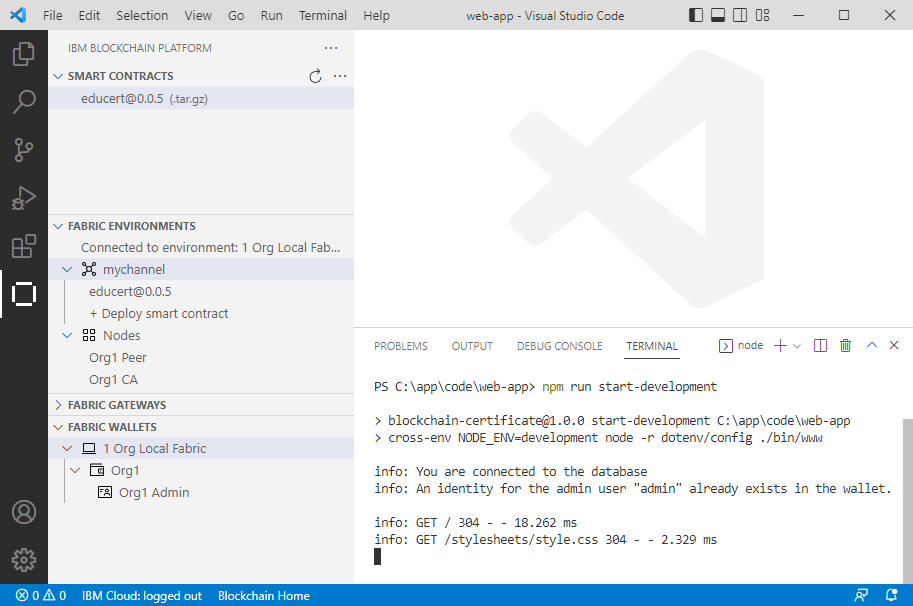
\includegraphics[width=.9\linewidth]{img/ide_start.PNG}
\caption{Chương trình Visual Studio Code}
\label{fig:ide_start}
\end{figure}

\section{Ứng dụng Web}

Giao diện ứng dụng web hoạt động tại địa chỉ http://localhost:3000/ như hình \ref{fig:main_vbcc}. 

\begin{figure}[H]
\centering
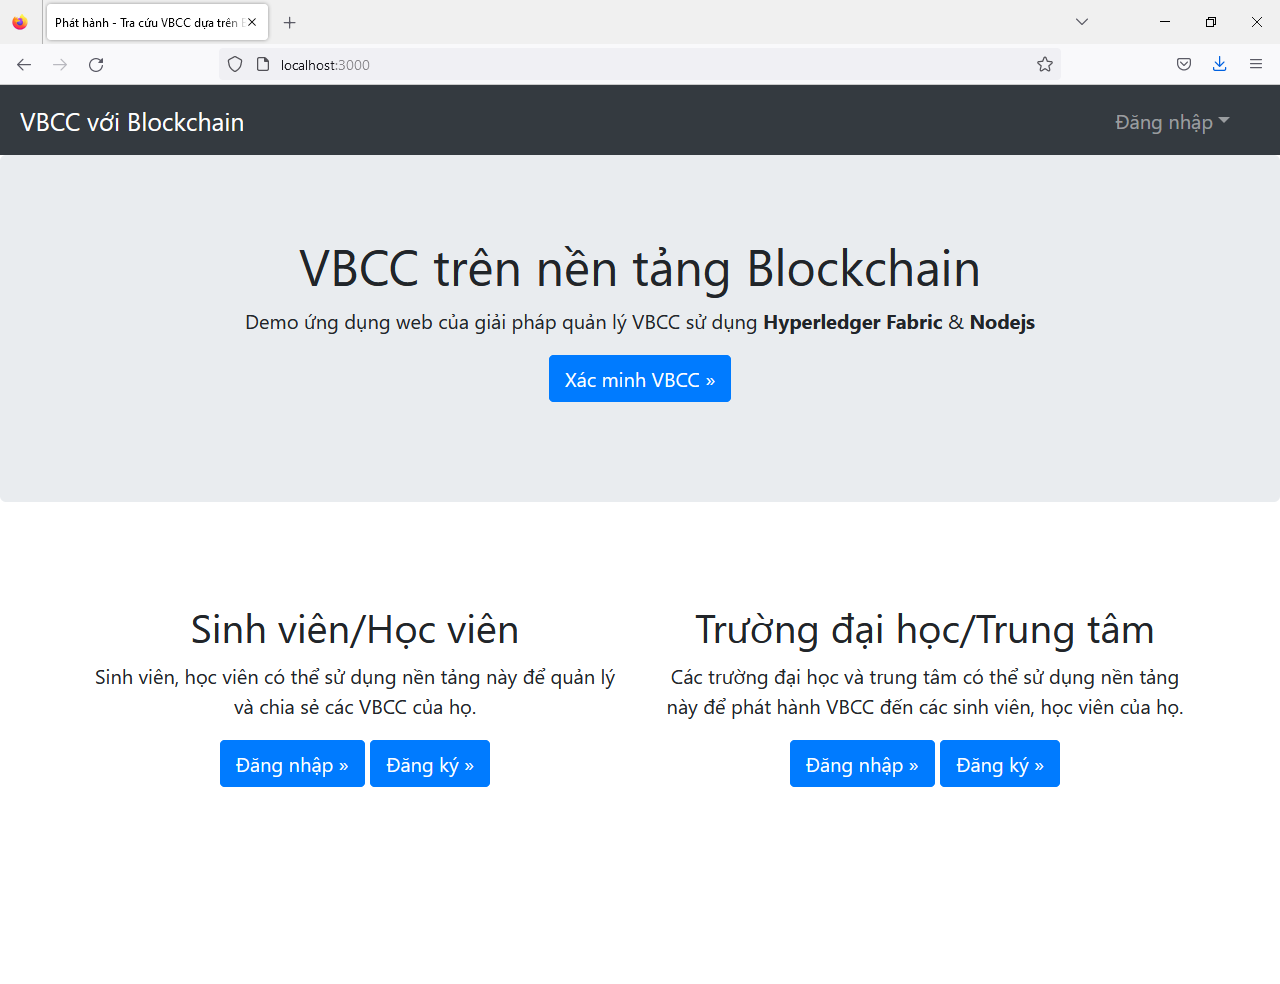
\includegraphics[width=.9\linewidth]{img/main_vbcc.png}
\caption{Giao diện hệ thống}
\label{fig:main_vbcc}
\end{figure}

\textbf{Màn hình chức năng quản lý của Trường, trung tâm}, hình \ref{fig:manhinh_bangdieukhien}

\begin{figure}[H]
\centering
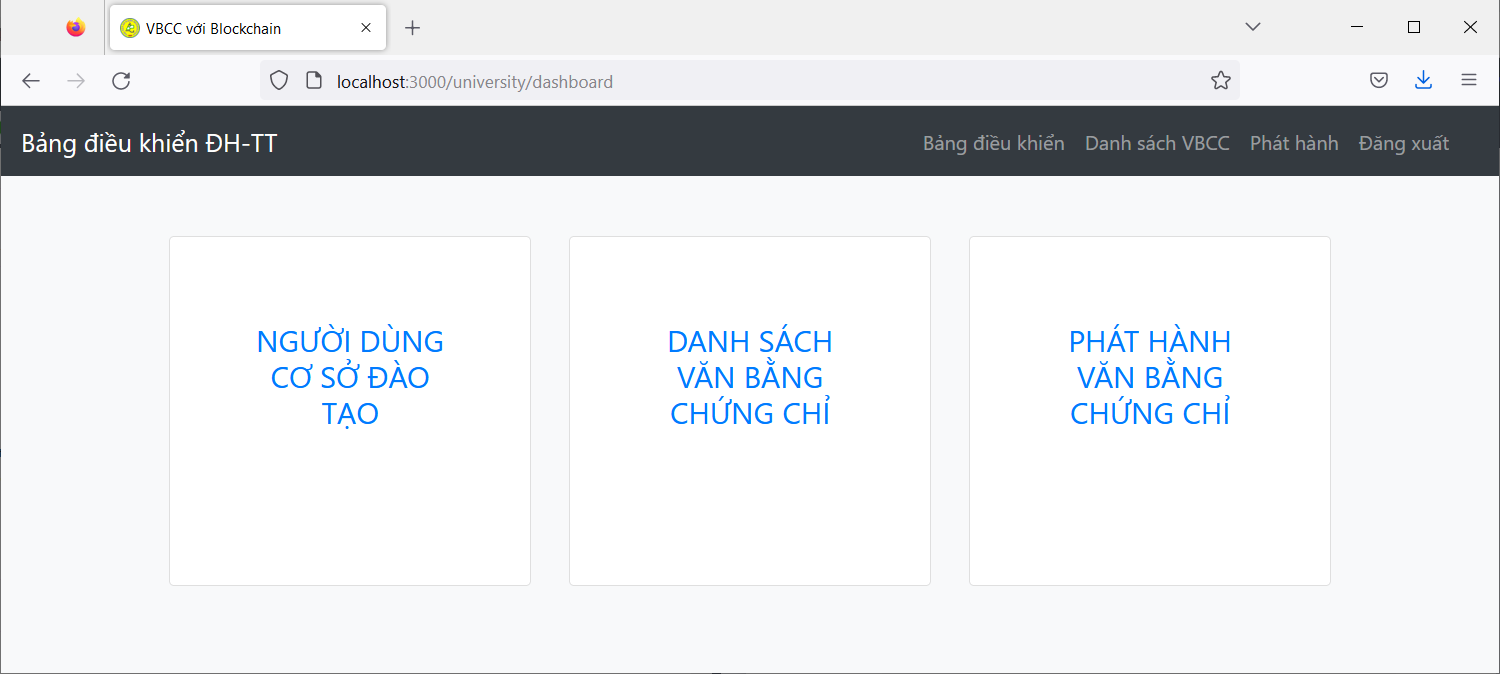
\includegraphics[width=.9\linewidth]{img/manhinh_bangdieukhien.png}
\caption{Màn hình chức năng của Cơ sở đào tạo}
\label{fig:manhinh_bangdieukhien}
\end{figure}

\emph{Màn hình hiển thị người dùng của cơ sở đào tạo}, hình \ref{fig:manhinh_danhsachnguoidungcsdt}

Trường thực hiện đăng nhập sử dụng hệ thống. Sau đó, chọn Bảng điều khiển, tiếp theo chọn người dùng cơ sở đào tạo để hiển thị danh sách người dùng của cơ sở đào tạo trong hệ thống.

\begin{figure}[H]
\centering
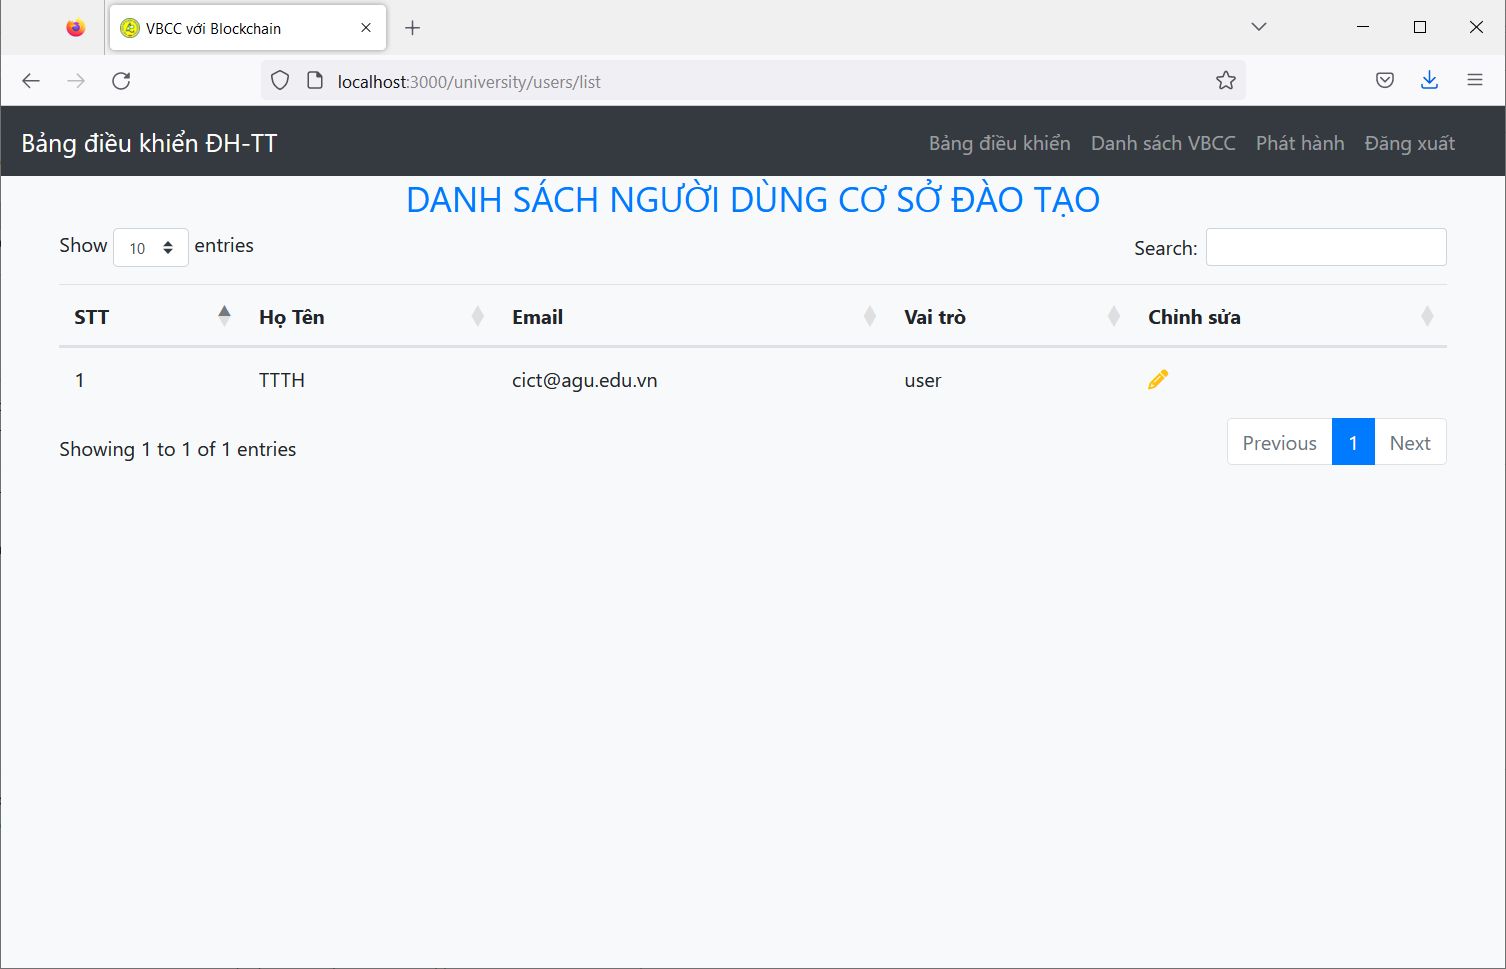
\includegraphics[width=.9\linewidth]{img/manhinh_danhsachnguoidungcsdt.png}
\caption{Màn hình hiển thị người dùng của cơ sỏ đào tạo}
\label{fig:manhinh_danhsachnguoidungcsdt}
\end{figure}

\emph{Màn hình hiển thị danh sách VBCC đã cấp cho sinh viên}, hình \ref{fig:manhinh_danhsachvbcc}

Trường thực hiện đăng nhập sử dụng hệ thống.
Sau đó, chọn Danh sách VBCC để hiển thị danh sách VBCC đã cấp cho sinh viên.

\begin{figure}[H]
\centering
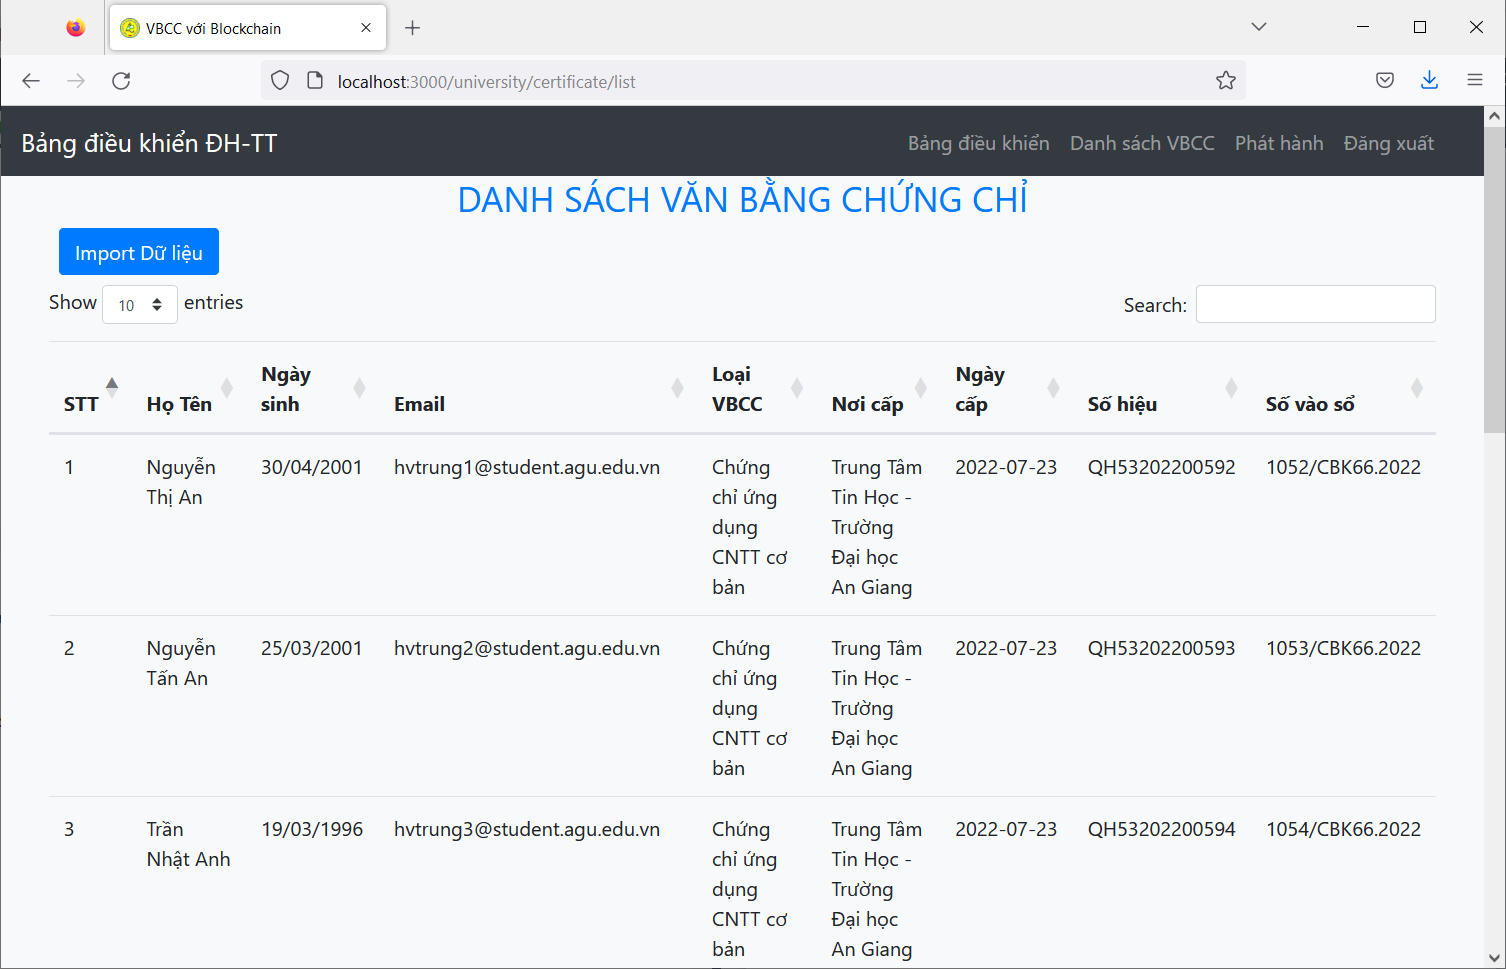
\includegraphics[width=.9\linewidth]{img/manhinh_danhsachvbcc.PNG}
\caption{Màn hình danh sách các VBCC đã cấp}
\label{fig:manhinh_danhsachvbcc}
\end{figure}


\emph{Màn hình cấp danh sách VBCC nhập từ file Excel}, 

Trường thực hiện đăng nhập sử dụng hệ thống. Sau đó, chọn Danh sách VBCC, chọn Import dữ liệu, hình \ref{fig:manhinh_importdulieu}.
\begin{figure}[H]
\centering
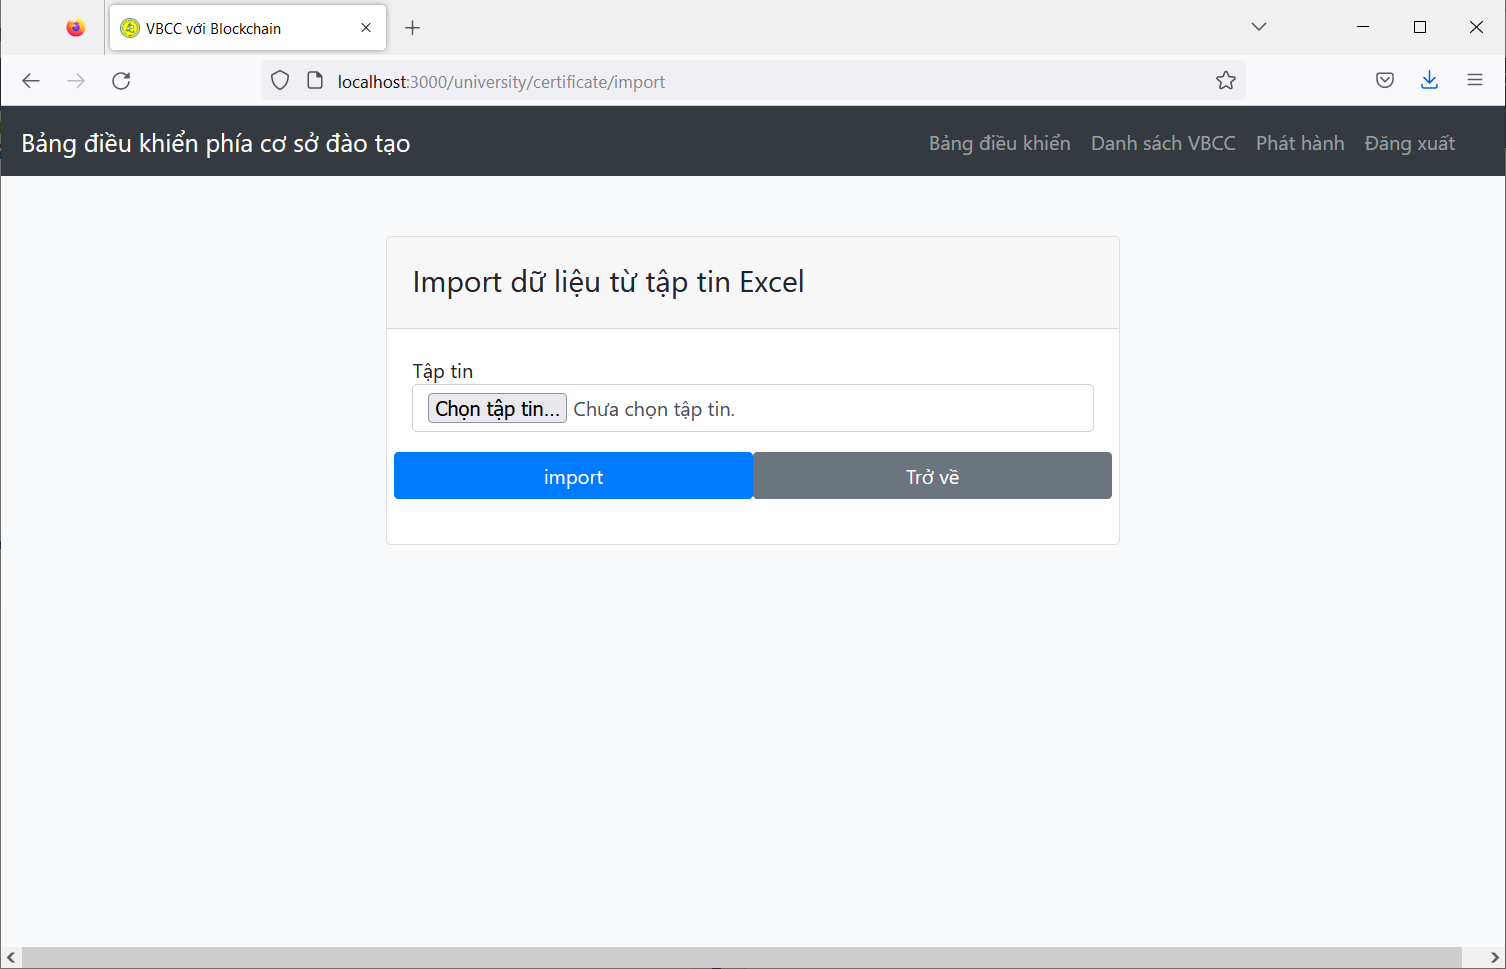
\includegraphics[width=.9\linewidth]{img/manhinh_importdulieu.PNG}
\caption{Màn hình cấp VBCC theo file Excel danh sách VBCC}
\label{fig:manhinh_importdulieu}
\end{figure}

File Excel danh sách VBCC như hình \ref{fig:excel}, gồm có thông tin VBCC và tài khoản sinh viên là email, mật khẩu sẽ được tạo trong hệ thống.

\begin{figure}[H]
\centering
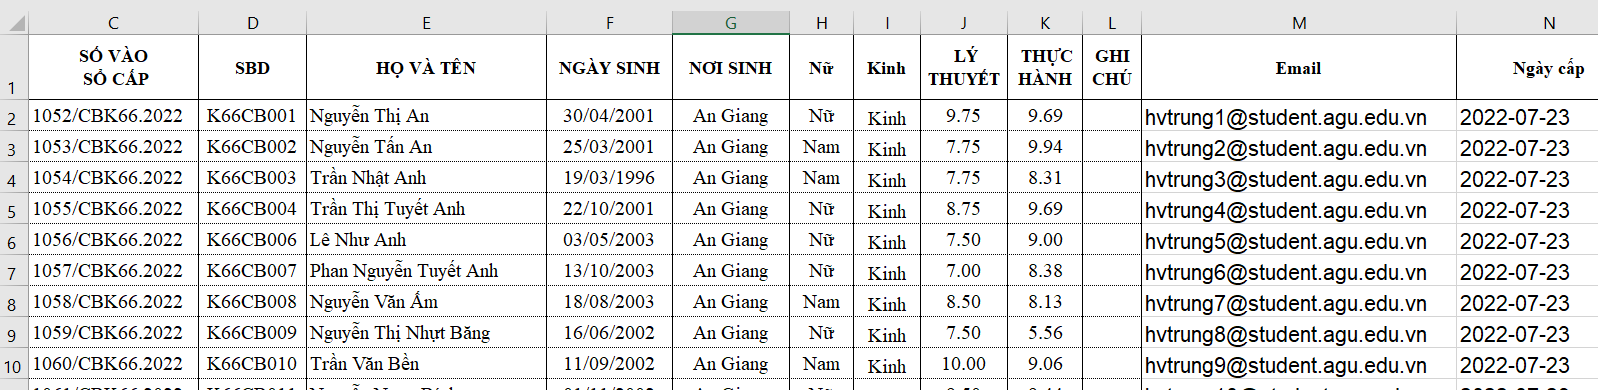
\includegraphics[width=.9\linewidth]{img/excel.png}
\caption{File Excel danh sách VBCC}
\label{fig:excel}
\end{figure}

\emph{Màn hình cấp VBCC cho sinh viên}, hình \ref{fig:tt_phathanh}

Trường thực hiện đăng nhập sử dụng hệ thống. Sau đó, chọn chức năng phát VBCC. 

Sau đó nhập thông tin VBCC, trong đó email sinh viên cần tồn tại trước trong hệ thống.

\begin{figure}[H]
\centering
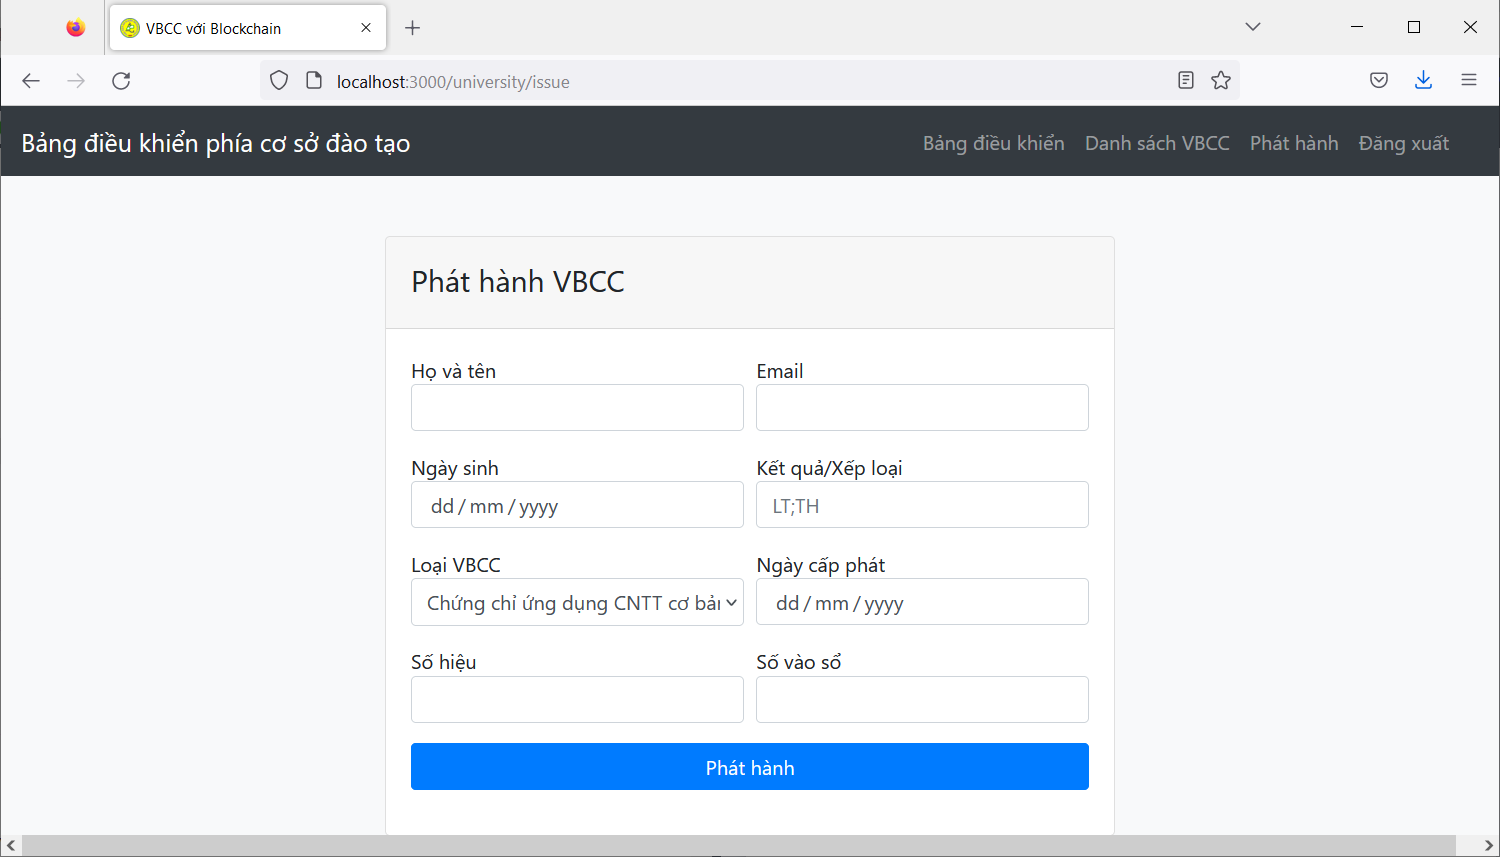
\includegraphics[width=.9\linewidth]{img/tt_phathanh.PNG}
\caption{Màn hình cấp VBCC cho sinh viên}
\label{fig:tt_phathanh}
\end{figure}

\textbf{Màn hình chức năng của sinh viên, học viên}

\emph{Màn hình đăng ký tài khoản}, hình \ref{fig:std_new}

Sinh viên nhập thông tin đăng ký, gồm có họ tên, email, mật mã đăng nhập.

\begin{figure}[H]
\centering
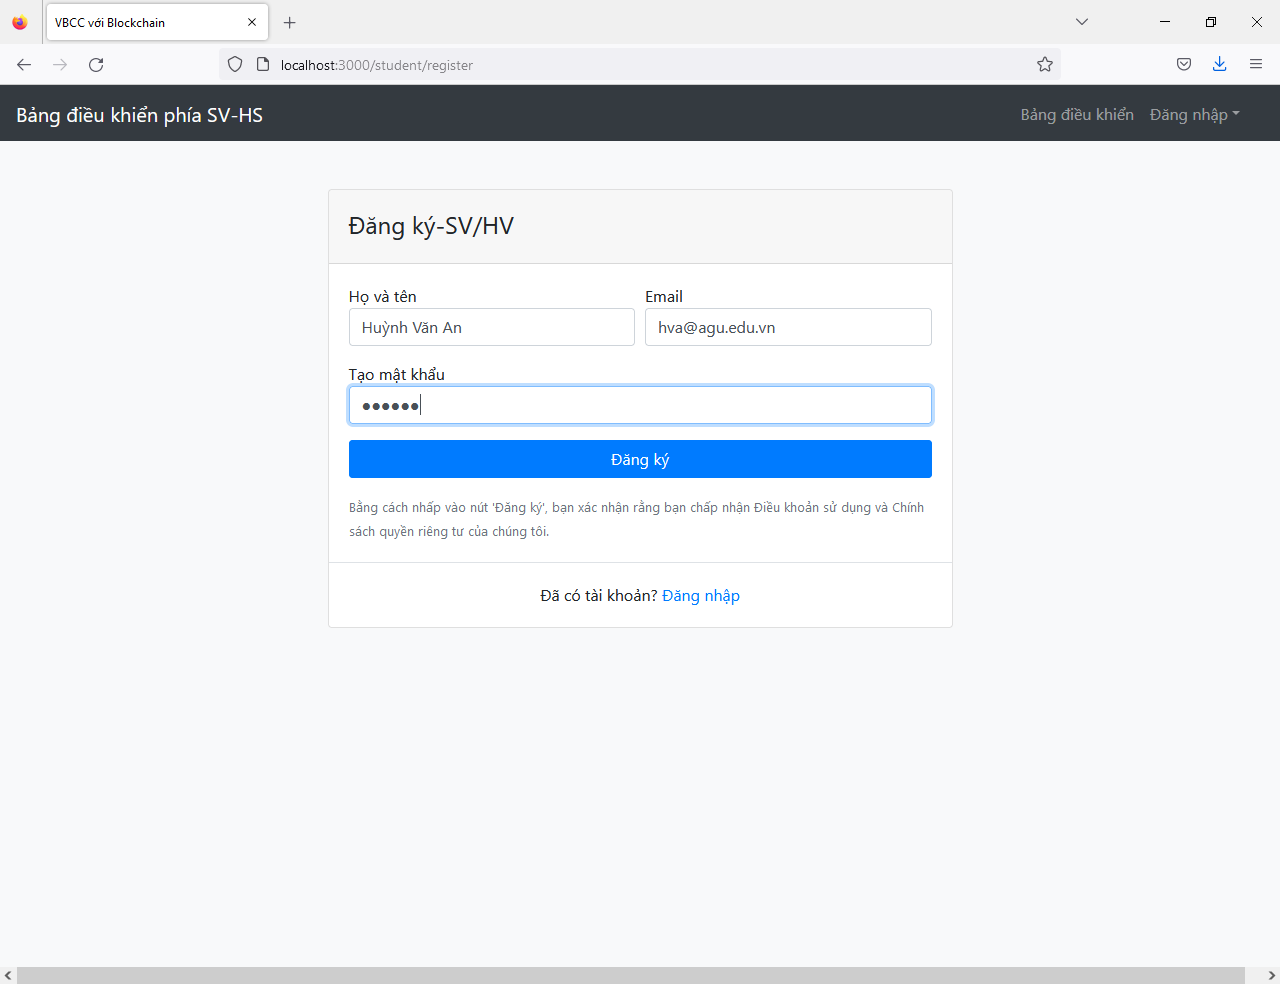
\includegraphics[width=.9\linewidth]{img/std_new.PNG}
\caption{Màn hình đăng ký tài khoản sinh viên}
\label{fig:std_new}
\end{figure}


\emph{Màn hình xem các VBCC đã nhận}, hình \ref{fig:sv_hva}

Sinh viên cần đăng nhập tài khoản để sử dụng hệ thống.
Sau khi đăng nhập tài khoản, chương trình sẽ hiển thị danh sách VBCC.
\begin{figure}[H]
\centering
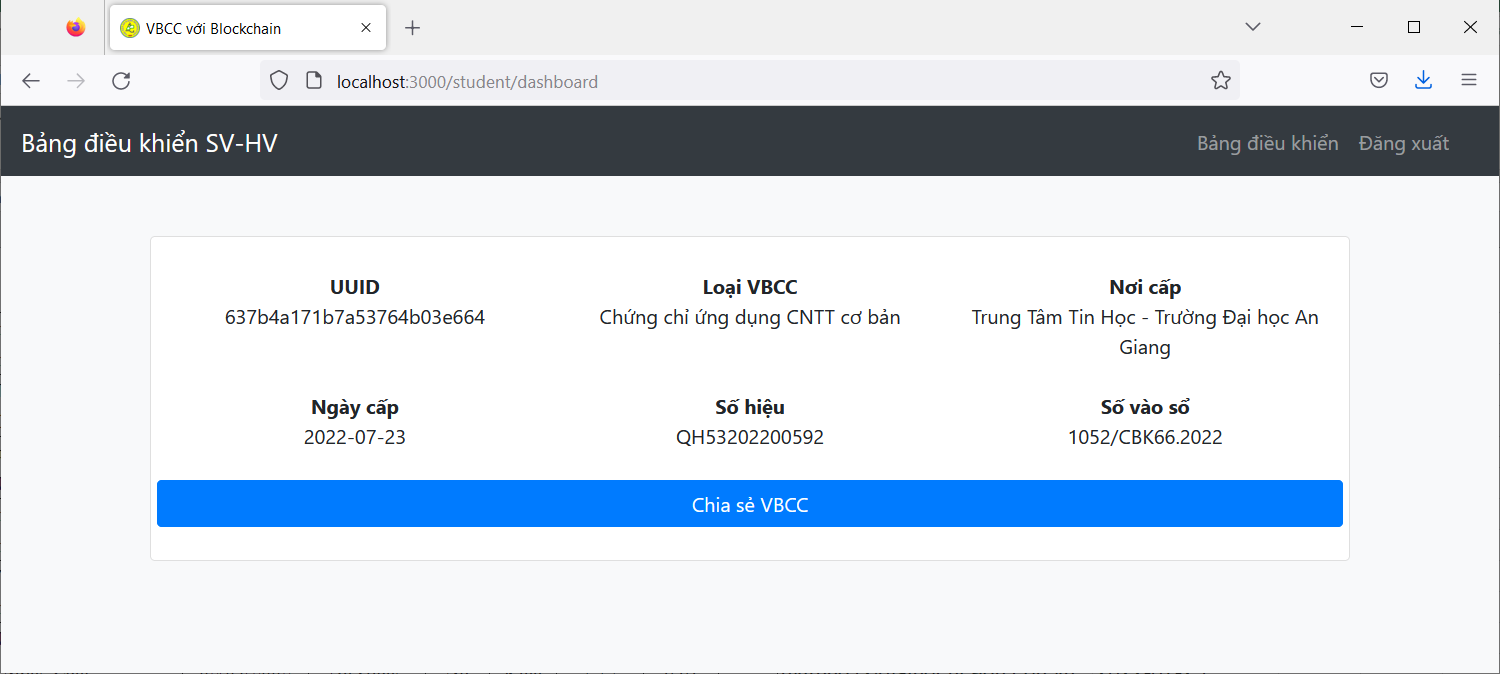
\includegraphics[width=.9\linewidth]{img/sv_hva.PNG}
\caption{Màn hình xem các VBCC đã nhận}
\label{fig:sv_hva}
\end{figure}

\emph{Màn hình chia sẻ VBCC đã nhận}, hình \ref{fig:sv_chiase}

Sinh viên cần đăng nhập tải khoản để sử dụng hệ thống.
Sinh viên chọn chức năng chia sẻ VBCC, và chọn những thông tin cá nhân cần chia sẻ. Sau đó chọn Tạo minh chứng.

\begin{figure}[H]
\centering
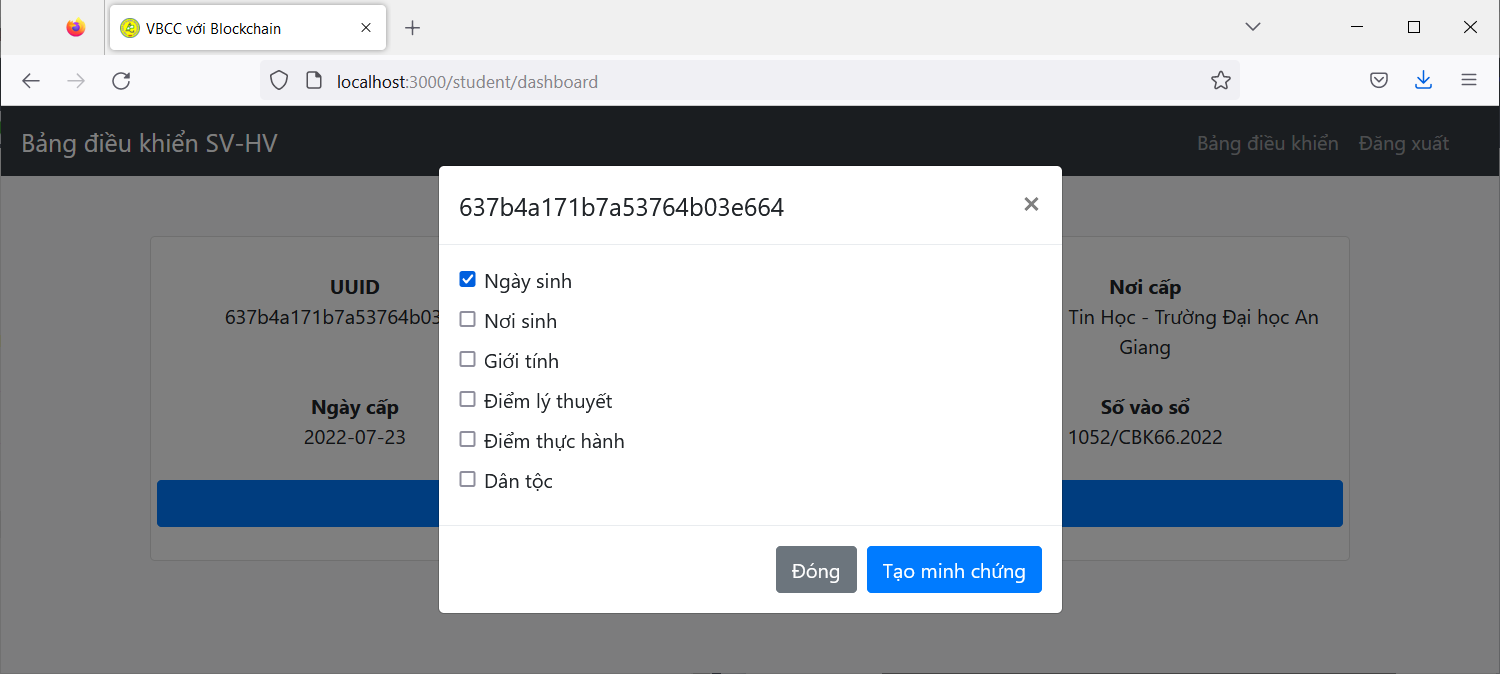
\includegraphics[width=.9\linewidth]{img/sv_chiase.PNG}
\caption{Màn hình chia sẻ thông tin VBCC}
\label{fig:sv_chiase}
\end{figure}

Sinh viên chép minh chứng gửi cho Đơn vị xác minh VBCC, hình \ref{fig:sv_minhchung}

\begin{figure}[H]
\centering
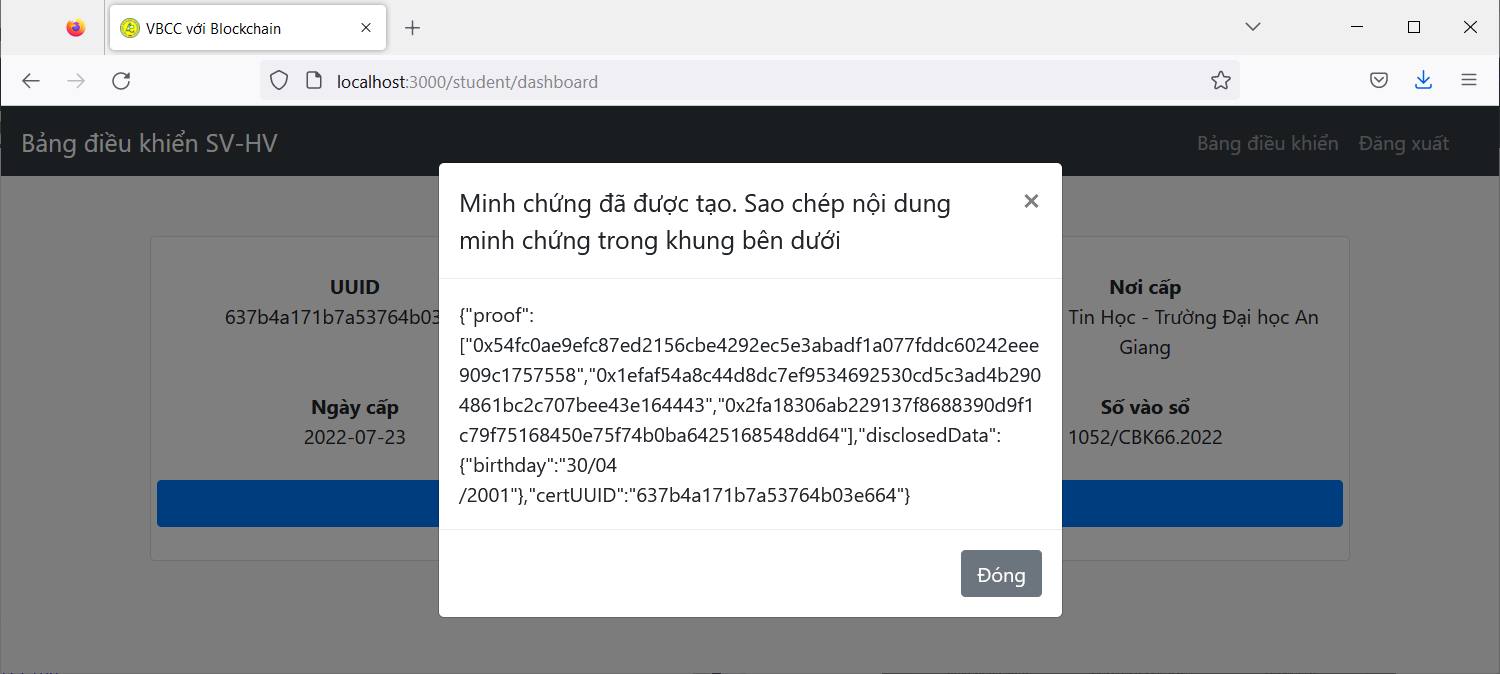
\includegraphics[width=.9\linewidth]{img/sv_minhchung.PNG}
\caption{Màn hình hiển thị minh chứng xác thực VBCC}
\label{fig:sv_minhchung}
\end{figure}

\textbf{Màn hình chức năng của Đơn vị xác minh VBCC}, hình \ref{fig:manhinh_donvixacminh}
\begin{figure}[H]
\centering
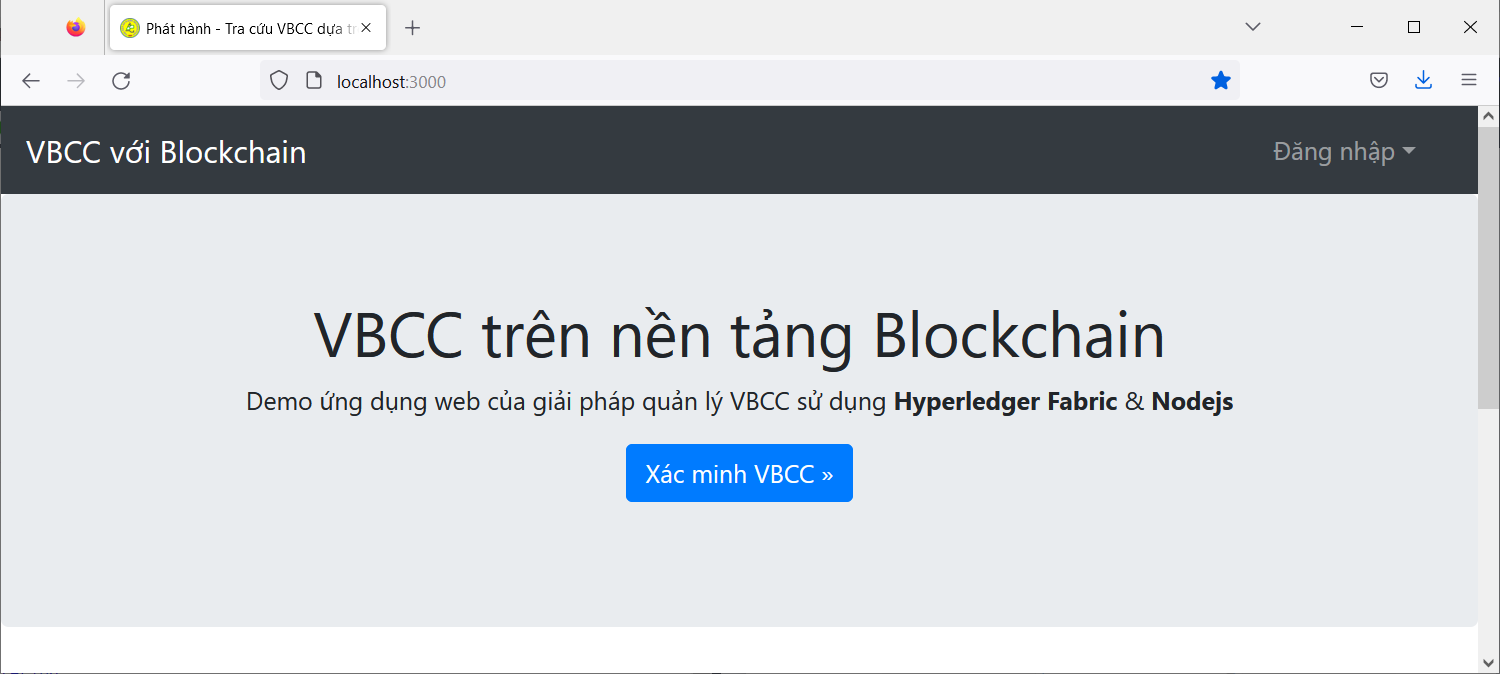
\includegraphics[width=.9\linewidth]{img/manhinh_donvixacminh.PNG}
\caption{Màn hình xác minh VBCC}
\label{fig:manhinh_donvixacminh}
\end{figure}
Hình \ref{fig:manhinh_donvixacminh_vbegin} sau khi nhấn vào Xác minh VBCC

\begin{figure}[H]
\centering
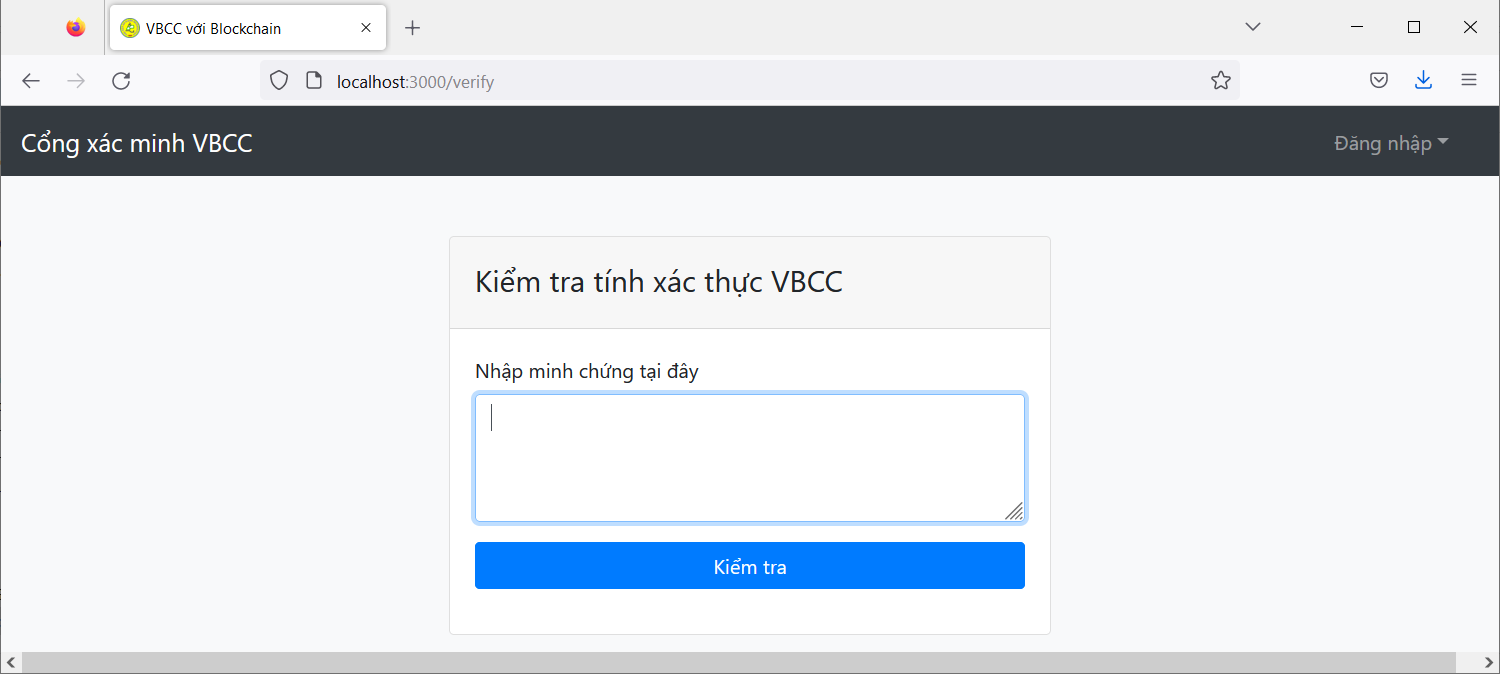
\includegraphics[width=.9\linewidth]{img/manhinh_donvixacminh_vbegin.PNG}
\caption{Màn hình nhập mã xác minh VBCC}
\label{fig:manhinh_donvixacminh_vbegin}
\end{figure}


Đơn vị nhận được minh chứng VBCC. 
Sau đó dán vào ô nhập minh chứng để kiểm tra.
Kết quả xác thực: nếu minh chứng đúng thì thông báo hợp lệ như hình \ref{fig:xacminh_hople} hoặc ngược lại thông báo không hợp lệ.
\begin{figure}[H]
\centering
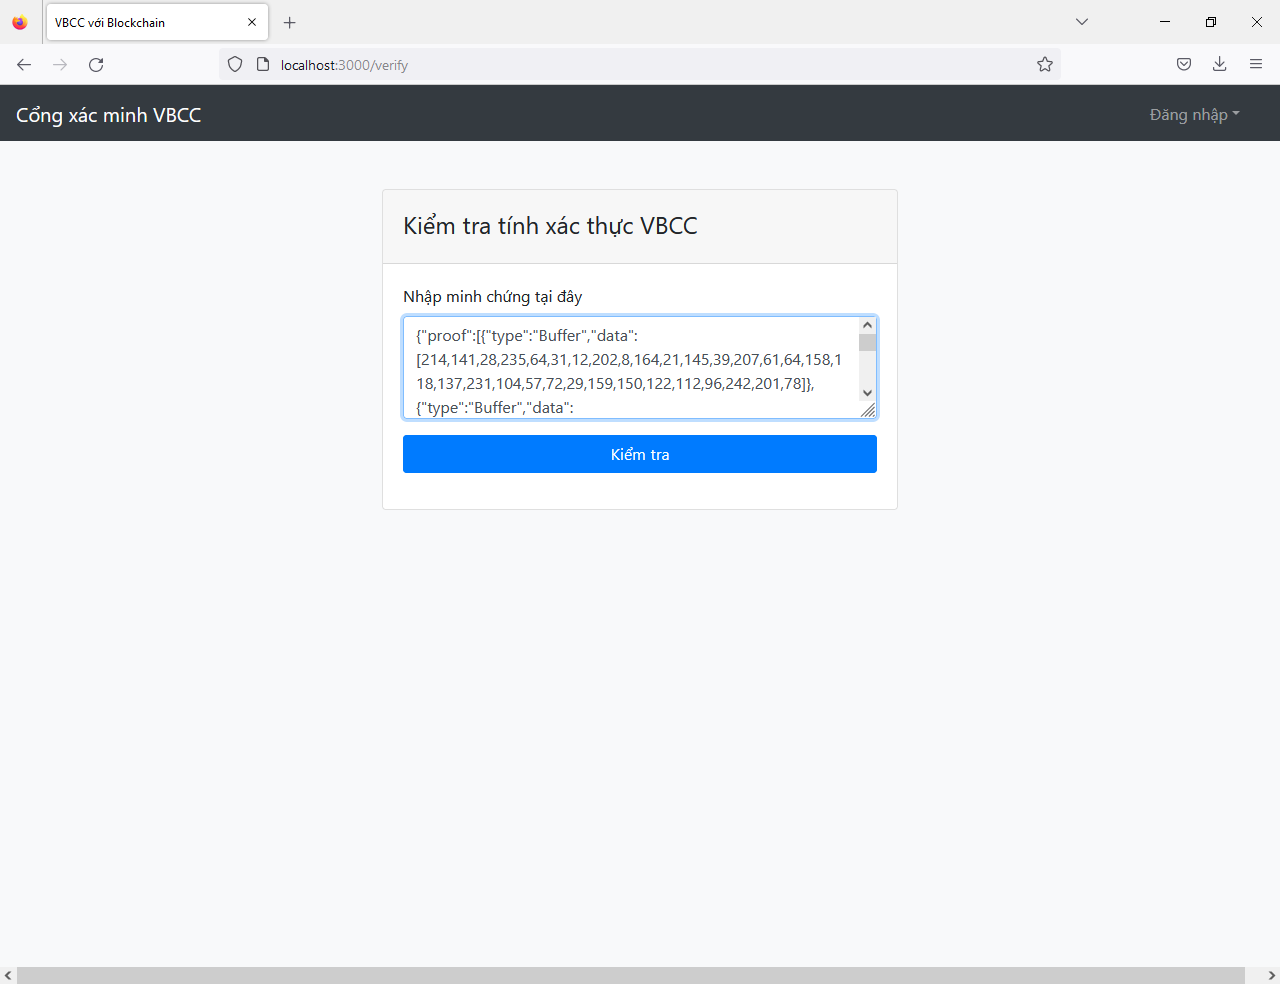
\includegraphics[width=.9\linewidth]{img/v_begin.PNG}
\caption{Màn hình sau khi nhập mã xác minh VBCC}
\label{fig:v_begin}
\end{figure}

\begin{figure}[H]
\centering
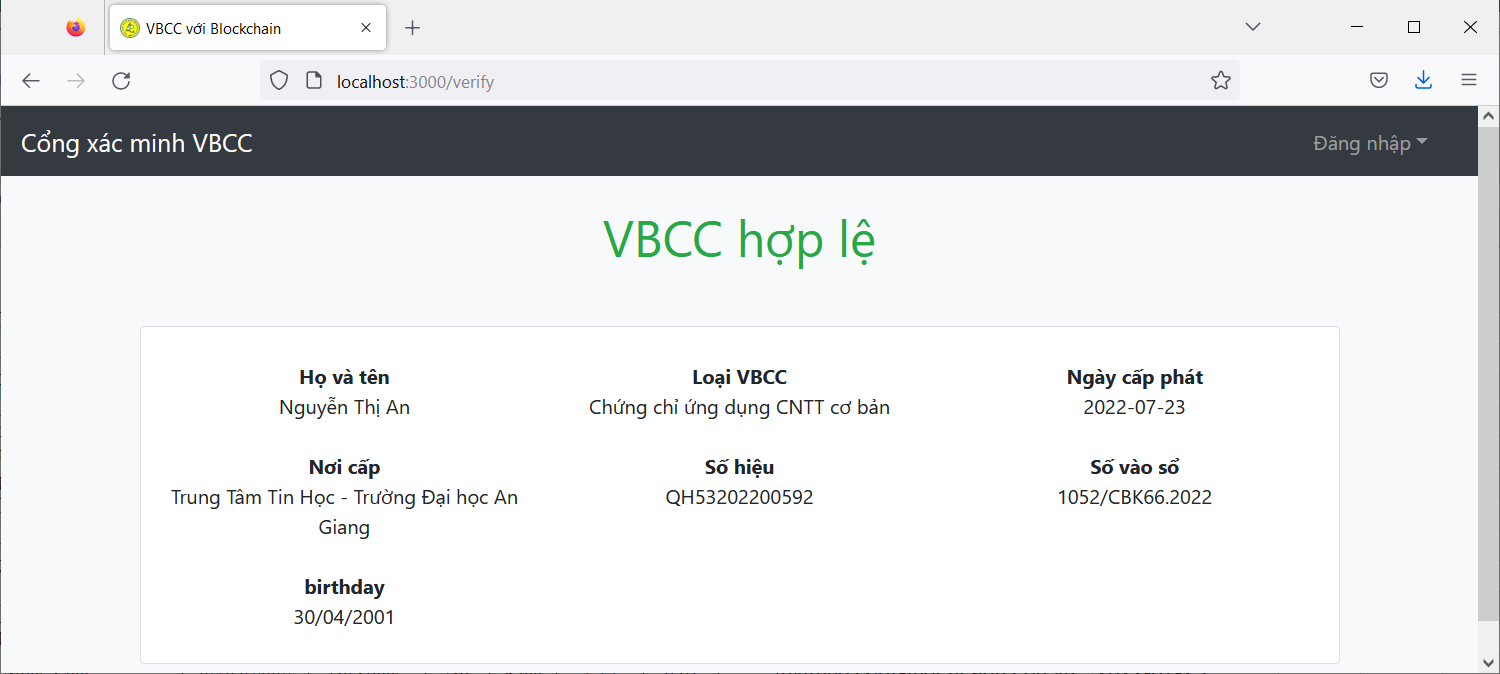
\includegraphics[width=.9\linewidth]{img/xacminh_hople.PNG}
\caption{Màn hình thông báo VBCC hợp lệ}
\label{fig:xacminh_hople}
\end{figure}

\section{Tiểu kết chương 4}

Chương 4 trình bày kết quả thực nghiệm hệ thống quản lý VBCC sử dụng công nghệ blockchain. Hệ thống thử nghiệm hoạt động trên máy tính cá nhân. Hệ thống quản lý VBCC có giao diện web với các chức năng chính cho người sử dụng như: (1) Trường quản lý và cấp VBCC; (2) Sinh viên nhận VBCC và chia sẻ thông tin VBCC; (3) Đơn vị xác thực VBCC. 
